\documentclass[12pt]{article}
\usepackage[utf8]{inputenc}
\usepackage[T1]{fontenc}
\usepackage{geometry}
\geometry{margin=1in}
\usepackage{hyperref}
\usepackage{enumitem}       
\usepackage{apacite}
\usepackage{csquotes}
\usepackage{graphicx}

\title{GDD (Game Design Document) for A2}
\author{Dylan Rumble-Smith}
\graphicspath{ {./media/} }

\setlength{\parindent}{0pt}
\setlength{\parskip}{1em}

\begin{document}
	{\setlength{\parskip}{0pt}%
		\maketitle
		\bibliographystyle{apacite}
		\pagebreak
		\tableofcontents
		\pagebreak
		}
	
	\section{Introduction}
	In this document, I aim to explain the processes and logic behind the artifacts for my A2 project, while also discussing the culture and history of other games and genres. Additionally, I'll review video game laws and how developers and publishers adapted to them when releasing games.
	
	This document is to be used along with a copy of my video game, as this document will refer to mechanics within that game and explain the context and inner-workings of them.
	\subsection{Game Title}
	The title of the game I am making is Fringe, stylised as FRINGE in promotional material. The title of my game is directly related to its definition, as the word “fringe” is defined as:
	\begin{displaycquote}{fringeMirriamWebster}
		something that is marginal, additional, or secondary to some activity, process, or subject
	\end{displaycquote}
	
	One reason I picked this name is the similarity to the word fling, which promptly explains that within my video game, Fringe, the player is expected to fling themselves off walls and other surfaces within a region nearby them.
	
	Another reason I called the game Fringe is because of the other definition of the word fringe:
	\begin{displaycquote}{fringeMirriamWebster}
		something resembling a fringe: EDGE, PERIPHERY
	\end{displaycquote}
	
	This ties into the story of the game as the character is on the fringe of the law and has to be kept in check.
	
	\subsection{Genres, Subgenres, and Inspiration}
	To make it easy for consumers to find a game that they are seeking, like songs and TV, video games can also be sorted into genres and subgenres. Common genres include, but are not limited to, action games, adventure games, puzzle games, and simulation games.
	
	These genres also have subgenres as well; for example, subgenres for the action genre may include platformer games, shooter games, fighting games, and survival games. These subgenres allow for more specific labelling of games.
	\newpage
	One game I am inspired by is Mirror’s Edge: A video game released in 2008. The game follows the main character Faith, a runner in the society of Mirror’s Edge. These runners carry sensitive documents with them and act as a courier. \cite{mirrorsEdgeGamespot}
	
	The game is labelled as an action adventure game, which is a type of action game. This means that it has action, and it has an adventurous theme.
	
	\begin{figure}[h]
		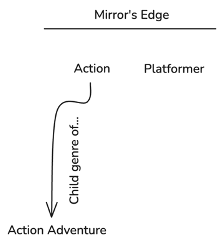
\includegraphics{mirrorsEdgeGenres}
		\centering
		\caption{A diagram showing the genres of Mirror's Edge}
	\end{figure}
	
	Mirror’s Edge has numerous mechanics that it is famous for, such as wall jumping and wall sliding. These mechanics allow for adding complexity to the level design and make the game more interesting as the player can do more actions to complete a level.
	\pagebreak
	{\setlength{\parskip}{0pt}%
	\bibliography{references}
	}
	
\end{document}
